El proyecto que Traverso crea por defecto contiene 6 pistas vacías y se llama \emph{Untitled}. Vamos a lanzar Traverso e importar un archivo de audio para trabajar con el.

Necesitará un archivo de audio, o mejor un par de ellos, en un formato soportado por Traverso. Los puede importar desde cualquier lugar del disco duro, o colocarlos el el directorio de proyectos de Traverso, preferiblemente en ``Untitled/audiosources'', para mantener los directorios ordenados. En Traverso, pulse \sact{I} en una pista vacía, navegue hasta los archivos de audio, y seleccione uno de ellos. El clip de audio correspondiente aparecerá en la pista, y la forma de onda se dibujará pasados unos segundos (este tiempo es necesario para calcular la forma de onda la primera vez).

Para escuchar el audio importado, presionamos la barra espaciadora. Los VUmetros mostrarán el nivel de la señal de salida. Si los VUmetros no están visibles, haga que se muestren desde el menú ``Ver $\rightarrow$ VUmetros''. El clip se pone en estado mudo pulsando \sact{U} cuando el ratón está sobre el clip. Para quitar el estado mudo, presione \sact{U} de nuevo. Por cierto: cuando vea una letra entre esas llaves, significa que pulse esa tecla una vez. Si pone el cursor sobre una zona vacía de la pista y pulsa \sact{U}, se pone en mudo la pista entera, y sólo entonces el botón ``mudo'' se enciende!

Ahora vamos a partir el clip en dos. Ponga el ratón donde quiera que el clip se divida, y pulse \sact{X}. Inmediatamente ¡tenemos dos clips! Use el botón deshacer del menú para deshacer la última acción. El clip volverá a su estado anterior.

Para cambiar la ganancia de una pista o de un clip, se pone el ratón sobre el clip, y se pulsa mantenidamente la tecla G. El cursor cambiará a un símbolo de ganancia (\FigB\ \ref{fig_gaincursor}). Ahora se mueve el ratón verticalmente, y se puede ver cómo cambia la ganancia. La notación que se empleará en lo sucesivo para la pulsación mantenida de una tecla es \hact{G}. Al soltar la tecla G el cursor vuelve a su estado normal, y el clip o la pista quedan con la nueva ganancia. Si coloca el ratón en una zona vacía de la pista, es decir donde no haya ningún clip, o en el panel de la pista (donde están los botones ``Mudo'', ``Solo'' y ``Rec''), pulsando mantenidamente \hact{G} y moviendo el ratón se cambia la ganancia de la pista. En lugar de mover el ratón, pruebe a girar la rueda del ratón mientras mantiene \hact{G}. Esto cambia la ganancia en pasos muy pequeños. Todas estas acciones, como se aprecia en la Historia, pueden deshacerse y rehacerse. También puede seleccionar un punto cualquiera de la Historia para volver directamente al estado en que se encontraba la edición en ese punto.

\begin{figure}
 \centering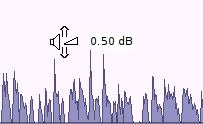
\includegraphics[width=0.4\textwidth]{../images/gain-cursor.png}
 \caption{El cursor se convierte en un símbolo de ganancia al hacer \hact{G}.}
 \label{fig_gaincursor}
\end{figure}

Hasta ahora hemos usado algunas acciones sencillas y fáciles de recordar, pero hay muchas más. Afortunadamente, tenemos menús contextuales para saber qué funciones están disponibles en cada momento para la pista o el clip de audio. Estos menús se muestran pulsando el botón derecho del ratón, o pulsando  \sact{Q} (como ya sabe, eso significa pulsar y soltar la tecla Q). El menú muestra las funciones disponibles, y cómo ejecutarlas con el teclado (\FigB\ \ref{fig_clipmenu}).

\begin{figure}
 \centering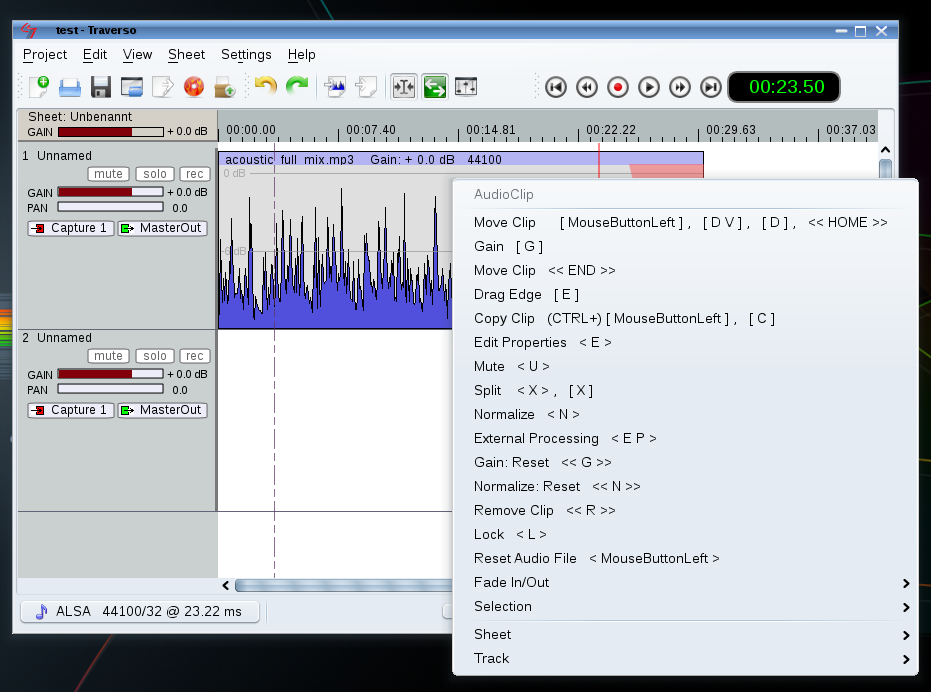
\includegraphics[width=\textwidth]{../images/clipmenu.png}
 \caption{Pulsando \sact{Q} o el botón derecho del ratón sobre un clip, se muestra el menú con las acciones disponibles.}
 \label{fig_clipmenu}
\end{figure}

Un clip de audio puede moverse ``arrastrándolo'' de la manera usual con el botón izquierdo del ratón, o manteniendo pulsada la tecla D mientras se mueve el ratón. Con la notación empleada esto es \hact{Botón Izquierdo}, y \hact{D}, respectivamente. Se puede mover libremente el ratón para colocar el clip donde se desee. Si el ratón se acerca a los límites de la ventana, la vista mostrada se desplazará automáticamente. Pruebe también las acciones \hact{Z} y \hact{S} para hacer zoom y para mover el deslizador horizontal.

Ya hemos aprendido dos tipos de acción: las acciones de teclado sencillas \sact{K}, y las acciones con pulsación mantenida \hact{K}. También hemos aprendido que las acciones de teclado actúan siempre sobre en objeto que está bajo el puntero del ratón. Pero antes de que empiece Vd. a explorar por sí mismo las posibilidades de Traverso, echemos un breve vistazo a algunas funciones más (elegidas sin un criterio particular).

Para restaurar a 0 dB la ganancia de un clip o de una pista, ponga el ratón sobre ella y pulse G dos veces rápidamente (notación \dact{G}). Como apreciará, esta acción primero restaura la ganancia a 0 dB, y si se ejecuta otra vez, la cambia a $-6$ dB. Llamadas sucesivas a esta función alternan la ganancia entre 0 y $-6$ dB. Funciona así tanto para las pistas como para los clips de audio.

